\documentclass[12pt,a4paper]{scrartcl}

\usepackage[utf8]{inputenc}
\usepackage[T1]{fontenc}
\usepackage[ngerman]{babel}

\usepackage[pdftex]{graphicx}
\usepackage{latexsym}
\usepackage{amsmath,amssymb,amsthm}
\allowdisplaybreaks
\usepackage{dsfont}
\usepackage{pifont}
\usepackage{nicefrac}
\usepackage{textcomp}
\usepackage{enumitem}
\usepackage{lmodern}

% Abstand obere Blattkante zur Kopfzeile ist 2.54cm - 15mm
\setlength{\topmargin}{-15mm}


% Umgebungen für Definitionen, Sätze, usw.
% Es werden Sätze, Definitionen etc innerhalb einer Section mit
% 1.1, 1.2 etc durchnummeriert, ebenso die Gleichungen mit (1.1), (1.2) ..
\newtheorem{Satz}{Satz}[section]
\newtheorem{Definition}[Satz]{Definition} 
\newtheorem{Lemma}[Satz]{Lemma}		   
                  
\numberwithin{equation}{section} 

\newcommand{\C}{\mathbb{C}} % komplexe
\newcommand{\K}{\mathbb{K}} % komplexe
\newcommand{\R}{\mathbb{R}} % reelle
\newcommand{\Q}{\mathbb{Q}} % rationale
\newcommand{\Z}{\mathbb{Z}} % ganze
\newcommand{\N}{\mathbb{N}} % natuerliche

\numberwithin{equation}{section}%

\newtheorem{thm}{Theorem}[section]%
\newtheorem{lem}[thm]{Lemma}%
\newtheorem{satz}[thm]{Satz}%
\newtheorem{prop}[thm]{Proposition}%
\newtheorem{algo}[thm]{Algorithmus}%

\newtheorem{cor}[thm]{Corollary}%
\theoremstyle{definition}
\newtheorem{dfn}[thm]{Definition}%
\newtheorem{bem}[thm]{Bemerkung}%
\newtheorem{exa}[thm]{Example}%
\newtheorem{bew}[thm]{Beweis}%


\begin{document}
  \pagestyle{empty}

\begin{titlepage}

	
\includegraphics[scale=0.45]{kit-logo.jpg} 
    \vspace*{2cm} 
\begin{center} \large 
    
   Masterarbeit
    \vspace*{2cm}

    {\huge External DLA}\\
    \vspace*{2.5cm}

    Tillmann Tristan Bosch
    \vspace*{1.5cm}

    10. März 2020
    \vspace*{3.5cm}


    Betreuung: Prof. Dr. Steffen Winter \\[1cm]
    Fakultät für Mathematik \\[1cm]
		Karlsruher Institut für Technologie
\end{center}
\end{titlepage}

\ \\
\newpage

\tableofcontents %Inhaltsverzeichnis

\newpage
\phantom \\
\newpage

  \pagestyle{headings}

\setcounter{page}{1}
\section{Einleitung}
External DLA beschreibt einen stochastischen Prozess, welcher zumindest in ähnlicher Form in natürlichen Prozessen beobachtbar ist. Er ähnelt zum Beispiel der fraktalen Gestalt eines sich kreisförmig ausbreitenden Risses einer Glasscheibe, oder eines Risses eines Kristallfluids wie in LCD Displays in alten Autoradios (siehe Fotos). Er kann auch in Schneeflocken oder in elektrostatischen Anhaftungen an Metallen beobachtet werden. Die Formalisierung solcher Prozesse ist sehr aktuell und die sehr konstruktive Definition erlaubten bisher nur mühsame Folgerungen über Struktur und Verhalten des Prozesses. Wir werden uns Modelle auf $\mathbb{Z}^2$, sowie auf anderen Graphen, darunter auch fraktale Graphen, anschauen, und außerdem versuchen, eine Approximation der bisherigen Definition zu finden, die grundsätzlich handlicher ist und auf einfachere Weise zu Erkenntnissen führt. Wir werden außerdem diese Arbeit mit einigen Python Simulationen begleiten. Der Code ist frei verfügbar auf Github. \\
\\

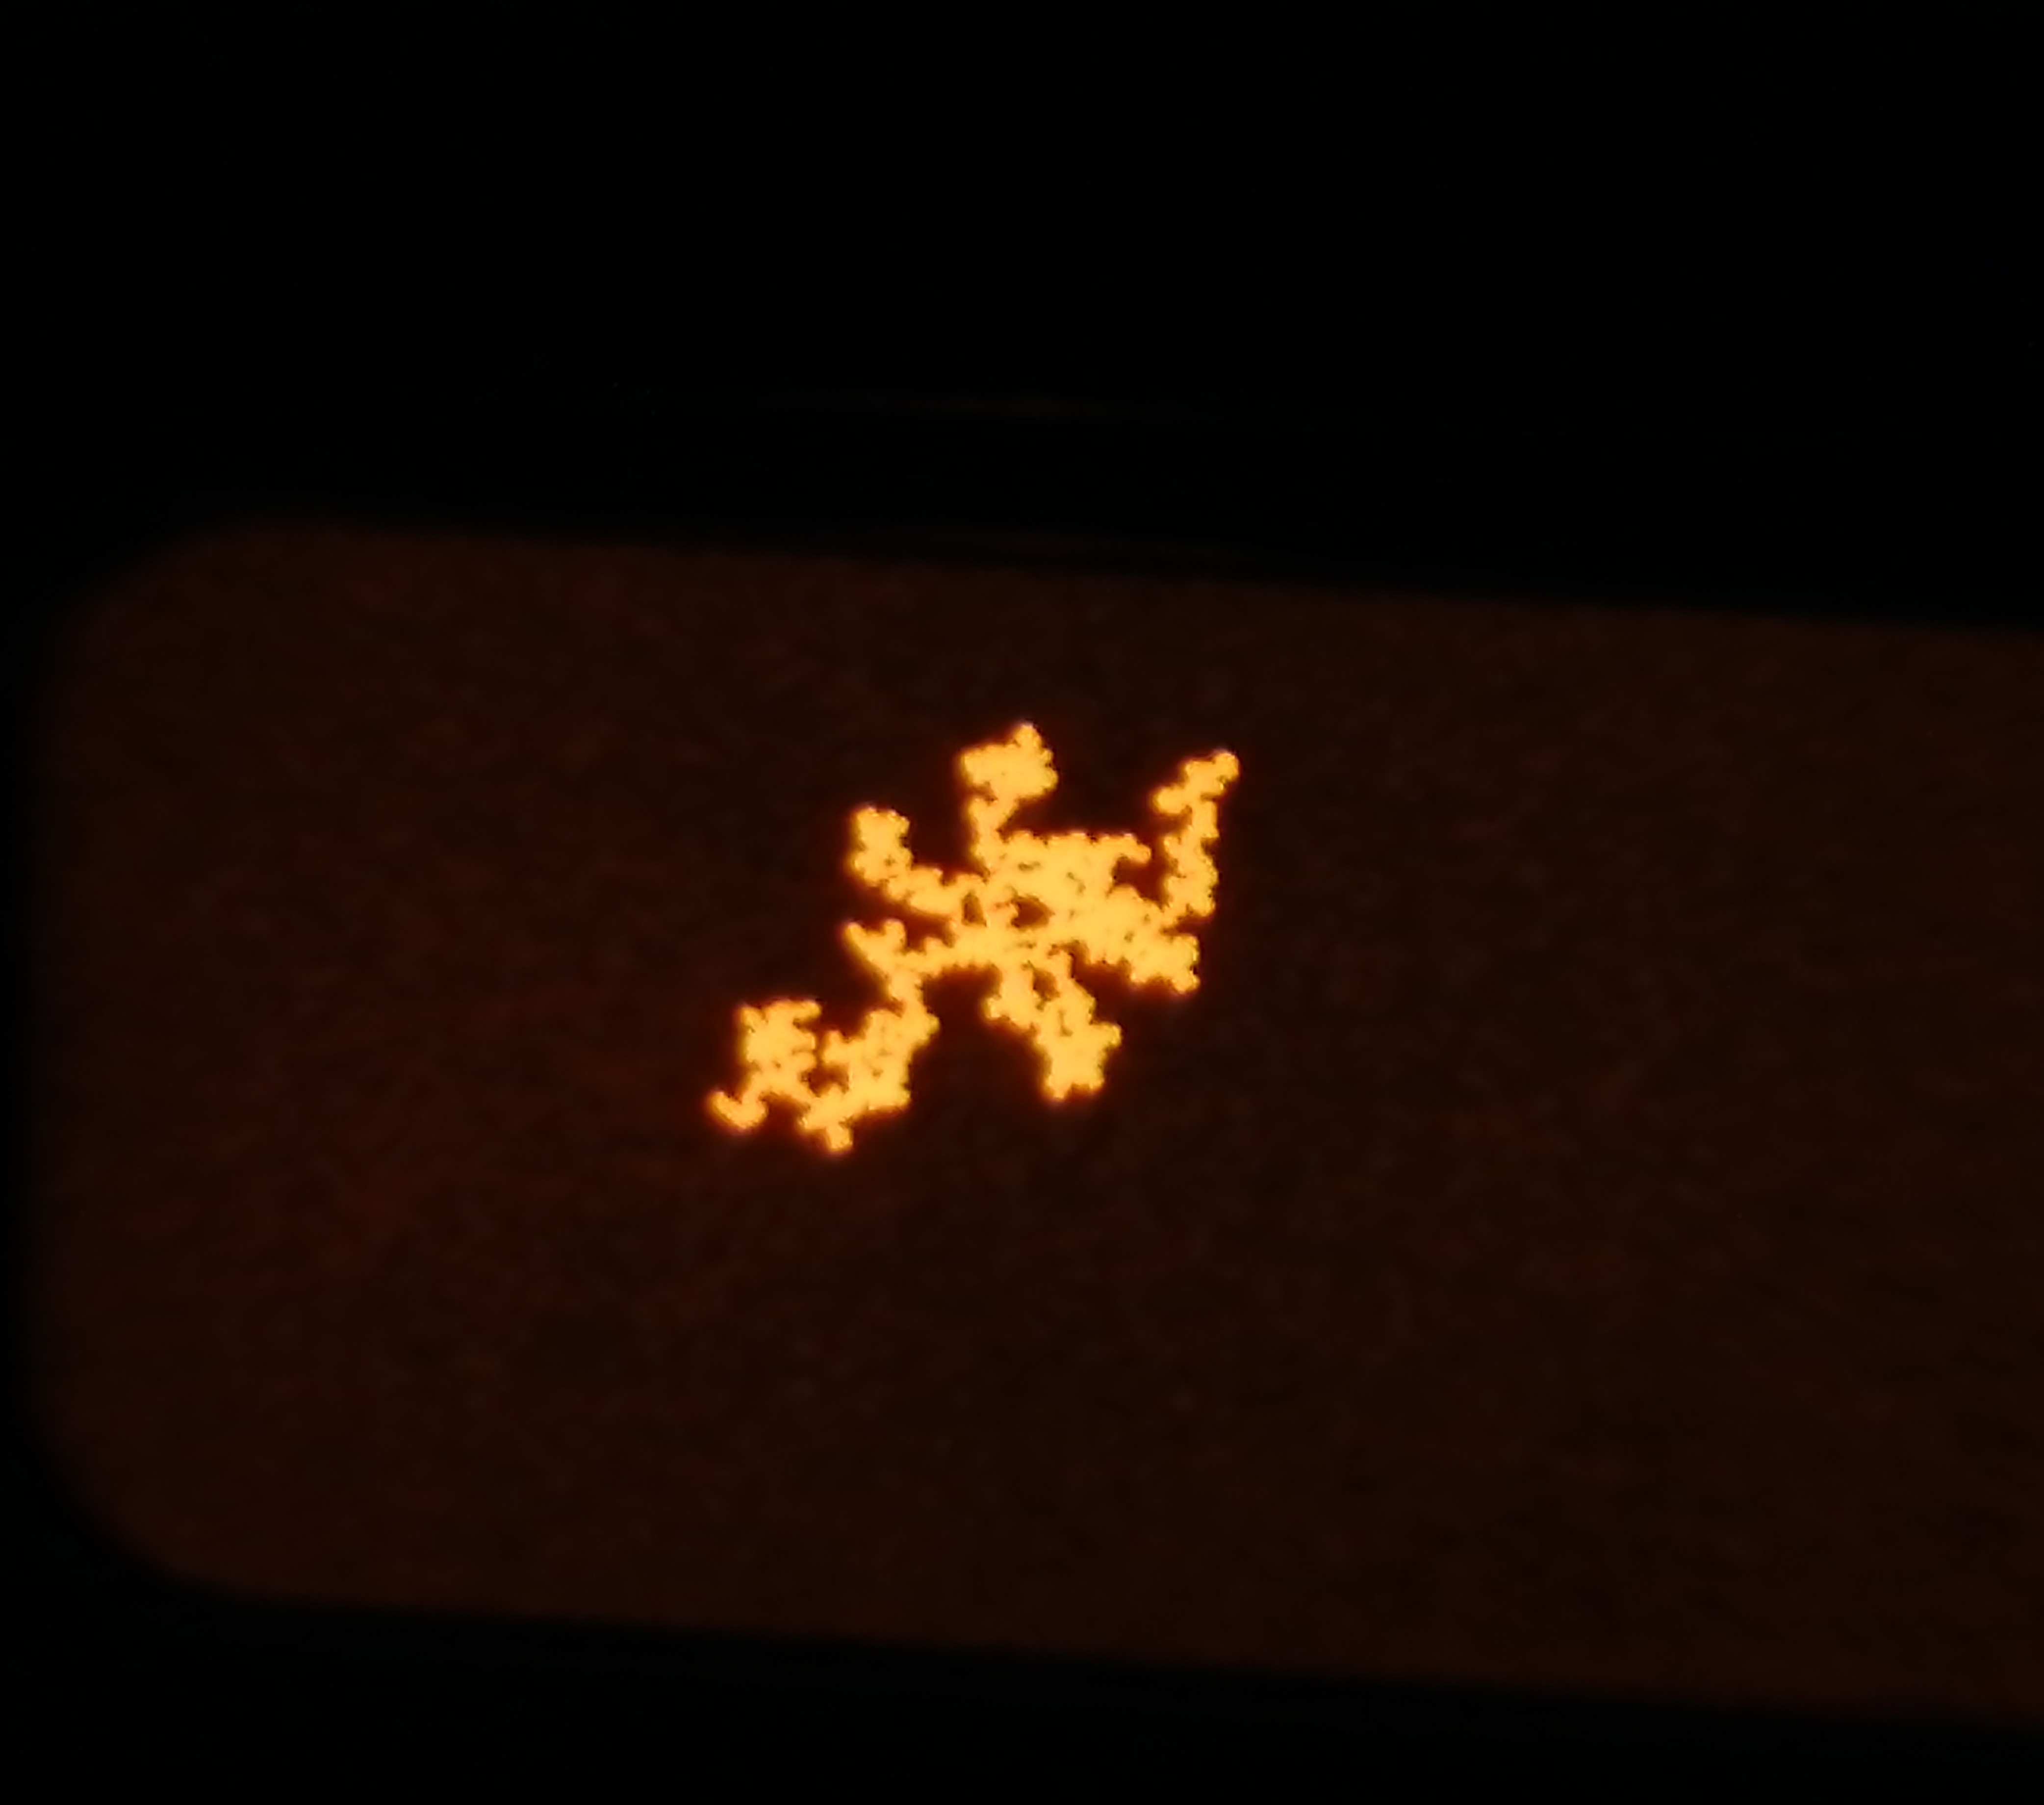
\includegraphics[scale=0.04]{display.jpg} 

\includegraphics[scale=0.091]{display2.jpg} 

\newpage

\begin{thebibliography}{Lam00}
\thispagestyle{empty}

\bibitem{Henze Skript}
N. Henze.
\emph{Maß und Wahrscheinlichkeitstheorie (Stochastik II)}.
Karlsruher Institut für Technologie, Karlsruhe, 2010

\end{thebibliography}

\newpage
  
\thispagestyle{empty}

\vspace*{8cm}


\section*{Erklärung}

Hiermit versichere ich, dass ich diese Arbeit selbständig verfasst und keine anderen als die angegebenen Quellen und Hilfsmittel benutzt, die wörtlich oder inhaltlich übernommenen Stellen als solche kenntlich gemacht und die Satzung des Karlsruher Instituts für Technologie zur Sicherung guter wissenschaftlicher Praxis in der jeweils gültigen Fassung beachtet habe. \\[2ex] 

\noindent
Karlsruhe, den 10. März 2020\\[5ex] 

\end{document}

